\section{Fjernbetjening}

For at øge sikkerheden er det besluttet at koble en fjernbetjening til dronen. Fjernbetjeningen skal udelukkende fungere som sikkerhed og vil ikke blive brugt til andre funktionaliteter.
For at kunne finde den bedst egnede fjernbetjening til projektet, er der opstillet nogle kriterier:

\begin{itemize}
	\item Antal kanaler.
	\item Pris.
	\item Rækkevidde.
\end{itemize}

Som udgangs punkt skal fjernbetjeningen minimum have 4 kanaler, disse skal bruges til styringen af dronen. 
Udover de 4 kanaler, ønskes en yderligere kanal. Denne kanal skal bruges til at afbryde den autonome del af dronen. 
Dette betyder at der ønskes en fjernbetjening med minimum 5 kanaler, helst fordelt som på figur~\ref{fig:fjernbetjening} 

\begin{figure}[H]
\centering
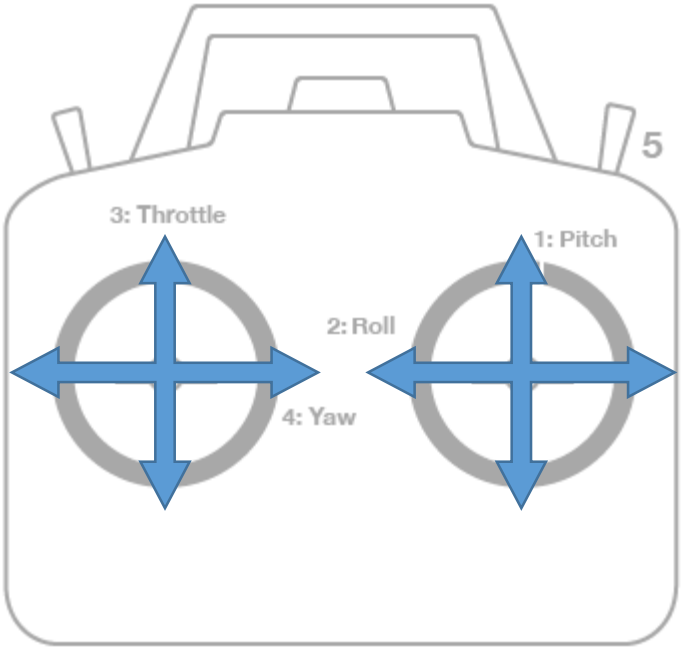
\includegraphics[width=0.5\textwidth]{Billeder/Fjernbetjening}
\caption{Fjernbetjening}
\label{fig:fjernbetjening}
\end{figure}

Hvor 4 af kanalerne bruges til selve styringen (Pitch, Roll, Throtte \& Yaw). Med disse kanaler er det muligt at få fuld kontrol over dronen.
I det fjernbetjeningen ikke har den største funktionalitet i systemet, er prisen en vigtig faktor. 

Rækkevidde er essentielt, idet det ikke hjælper at have en fjernbetjening hvis dronen er udenfor rækkevidden. 

Udefra valget af drone og hvilke erfaringer andre brugere havde med diverse fjernbetjeninger, blev det besluttet at købe en Spektrum DX5e 5 kanals fjernbetjening.
Fjernbetjeningen har 5 kanaler hvilket passer til kravene.